Finding minimal repairs has been shown to be NP-Complete even for FDs only \cite {Chiang}.
Moreover, finding minimal repairs for DCs and numerical values only is known to be MaxSNP-hard \cite{Bertossi}.
The work in \cite{XuChu} proposes an approximate holistic algorithm that is capable of generating nearly-optimal repairs for a given set of DCs.
The algorithm we propose for generating sapmle repairs for DCs is built upon two ideas: first, we try to generate a repair in a holistic manner as proposed in \cite{XuChu}, Second, we uses the
idea of generating random samples from the space of repairs, introduced in \cite{Beskales_sampling}.
Before going into the algorithm specifications, we will first see why the two of the above ideas cannot solve the problem alone.

\subsection{Previous Approaches}
First we will see why the repair sampling approach described in \cite{Beskales_sampling} is not self-sufficient to generate repairs for Denial-Constraints as well.
The idea in \cite{Beskales_sampling} is to grow the set of clean cells by merging the cells belonging to same equivalence class.
It is easy to build equivalence classes in case of FDs and CFDs, in other words when the set of predicates $B = \{ =, \neq\}$, 
but the equivalence class cannot be determined when the predicates are more loose, such as from set $B = \{ =, \neq\, <, >, \leq, \geq, \approx \}$.

Second, the approximate holistic algorithm in \cite{XuChu}, has two issues due to which it cannot be used for generating repairs.
One, the approximate algorithm uses minimum vertex cover (MVC) to find an approximately minimal repair, but it still does not gaurantee to cover all cardinality-Minimal space.
For example, consider the data instance given in  Table \ref{tab:eg1}, the MVC for the conflict hyper-edges is set $\{t_1.C, t_2.C and t_4.C\}$.
The holistic algorithm will pick one cell from MVC, say $t_2.C$ and form a frontier set and generate a repair expression for it.
The output repair from this will be the first repair in Table \ref{tab:eg2}, i.e. $t_1.C = t_2.C = t_3.C = t_4.C = 5$.
Although the cardinality-minimal repair is the second repair in Table \ref{tab:eg2}, i.e. $t_1.C = t_2.C = 3,t_4.D = V \leq 3$.
This cardinality-Minimal repair could have been acheived if the algorithm would have picked up cell $t_4.D$ first (that is not in MVC) and then $t_2.C$ to generate repair, we will show this in more detail in Section \ref{}.

The other issue with the holistic approach is that, it can also generate repairs which are not even Set-Minimal.
The cell modifications governed by the repair expression can generate new violations which are hendled in the next iteration of the algorithm.
We will see an example where a series of new violations can end up generating a Not Set-Minimal repair.
Consider a database instance and a set of DCs as shown in figure \ref{fig:eg4}.
The dotted box represents a violation hyperedge of a conflict hypergraph (CH).
The MVC for a single hyperedge CH can be any cell in that hyperedge.
Say, algorithm chose cell $t_2.B$ as MVC and generates a repair, as shown in Figure \ref{fig:notSetMinEg}(i), but introduces a new violation.
In the next iteration cell $t_2.A$ is a part of MVC and Figure \ref{fig:notSetMinEg}(ii) is the repair with a new violation, and so on, 
Figure \ref{fig:notSetMinEg}(i-iv) shows the repair and new violations introduced at each step of the iteration.
Figure \ref{fig:notSetMinEgFinal} shows all the cells changed in the repair process.
Now observe that the value of cell $t_2.B$ can be reverted back to its original value 5, and the resulting repair is shown in Figure \ref{fig:notSetMinEgOther} which is still a valid repair.
This proves that the holistic data cleaning algorithm can generate repairs which are not Set-Minimal.

\begin{figure}
   \centering
   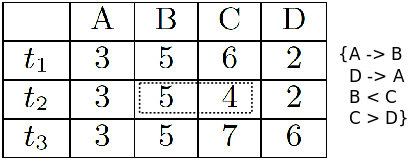
\includegraphics[scale=0.25]{eg4.png}
   \caption{Unclean database instance and a set of DCs. Dotted line is a hyperedge, showing violation.}
   \label{fig:eg4}
\end{figure}

\begin{figure}
   \centering
   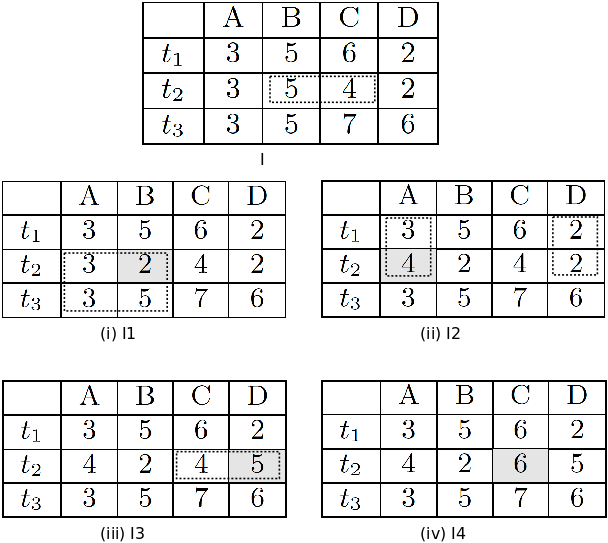
\includegraphics[scale=0.28]{notSetMinEg.png}
   \caption{Shows the repaired cell at each iteration and the new violation.}
   \label{fig:notSetMinEg}
\end{figure}

\begin{figure}
   \centering
   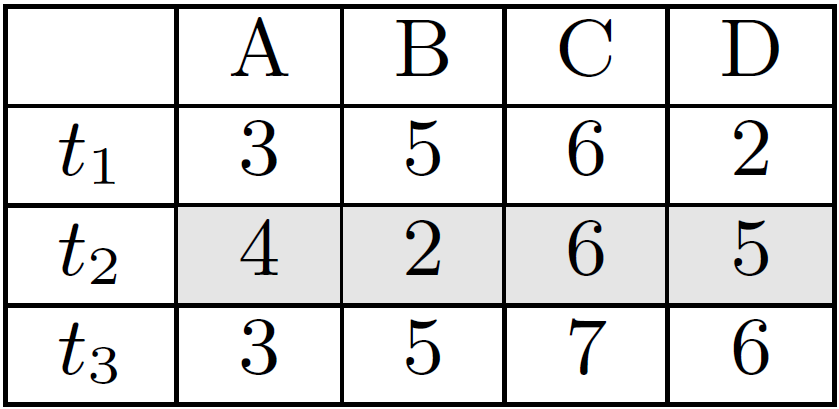
\includegraphics[scale=0.2]{notSetMinEgFinal.png}
   \caption{All the cell changed with respect to original I.}
   \label{fig:notSetMinEgFinal}
\end{figure}

\begin{figure}
   \centering
   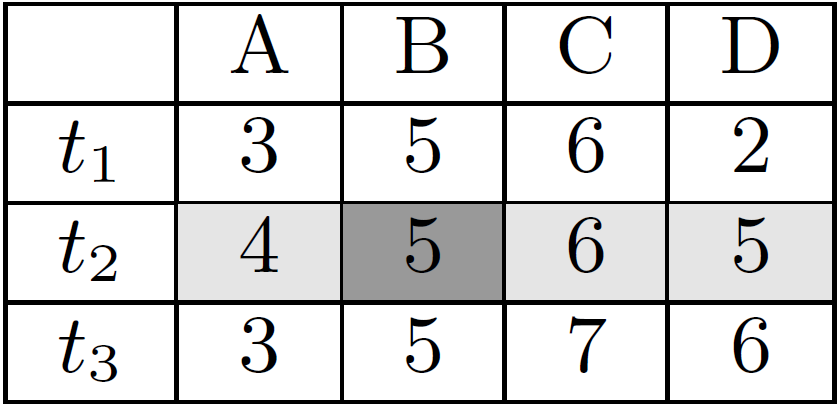
\includegraphics[scale=0.2]{notSetMinEgOther.png}
   \caption{Value of Cell $t_2.B$ can be reverted and the repair is still valid.}
   \label{fig:notSetMinEgOther}
\end{figure}

%
%\begin{table} \label{tab:eg1}
%\centering 
%\begin{tabular}{|c|c|c|c|c|}  \hline
%      & A & B & C & D 	\\ \hline
%   $t_1$ & 3 & 5 & 6 & 2 	\\ \hline
%   $t_2$ & 3 & 5 & 4 & 2 	\\ \hline
%   $t_3$ & 3 & 5 & 7 & 6 	\\ \hline
%\end{tabular}
%\caption{Sample Data.}
%\end{table}
%
%
%
%
%
%
%\begin{table} \label{tab:eg1}
%\centering 
%\begin{tabular}{|c|c|c|c|c|}  \hline
%      & A & B & C & D 	\\ \hline
%   $t_1$ & 3 & 5 & 6 & 2 	\\ \hline
%   $t_2$ & 3 & \cellcolor[gray]{0.9}2 & 4 & 2 	\\ \hline
%   $t_3$ & 3 & 5 & 7 & 6 	\\ \hline
%\end{tabular}
%\caption{Sample Data.}
%\end{table}
%
%\begin{table} \label{tab:eg1}
%\centering 
%\begin{tabular}{|c|c|c|c|c|}  \hline
%      & A & B & C & D 	\\ \hline
%   $t_1$ & 3 & 5 & 6 & 2 	\\ \hline
%   $t_2$ & \cellcolor[gray]{0.9}4 & 2 & 4 & 2 	\\ \hline
%   $t_3$ & 3 & 5 & 7 & 6 	\\ \hline
%\end{tabular}
%\caption{Sample Data.}
%\end{table}
%
%\begin{table} \label{tab:eg1}
%\centering 
%\begin{tabular}{|c|c|c|c|c|}  \hline
%      & A & B & C & D 	\\ \hline
%   $t_1$ & 3 & 5 & 6 & 2 	\\ \hline
%   $t_2$ & 4 & 2 & 4 & \cellcolor[gray]{0.9}5 	\\ \hline
%   $t_3$ & 3 & 5 & 7 & 6 	\\ \hline
%\end{tabular}
%\caption{Sample Data.}
%\end{table}
%
%\begin{table} \label{tab:eg1}
%\centering 
%\begin{tabular}{|c|c|c|c|c|}  \hline
%      & A & B & C & D 	\\ \hline
%   $t_1$ & 3 & 5 & 6 & 2 	\\ \hline
%   $t_2$ & 4 & 2 & \cellcolor[gray]{0.9}6 & 5 	\\ \hline
%   $t_3$ & 3 & 5 & 7 & 6 	\\ \hline
%\end{tabular}
%\caption{Sample Data.}
%\end{table}
%
%\begin{table} \label{tab:eg1}
%\centering 
%\begin{tabular}{|c|c|c|c|c|}  \hline
%      & A & B & C & D 	\\ \hline
%   $t_1$ & 3 & 5 & 6 & 2 	\\ \hline
%   $t_2$ & \cellcolor[gray]{0.9}4 & \cellcolor[gray]{0.9}2 & \cellcolor[gray]{0.9}6 & \cellcolor[gray]{0.9}5 	\\ \hline
%   $t_3$ & 3 & 5 & 7 & 6 	\\ \hline
%\end{tabular}
%\caption{Sample Data.}
%\end{table}
%
%\begin{table} \label{tab:eg1}
%\centering 
%\begin{tabular}{|c|c|c|c|c|}  \hline
%      & A & B & C & D 	\\ \hline
%   $t_1$ & 3 & 5 & 6 & 2 	\\ \hline
%   $t_2$ & \cellcolor[gray]{0.9}4 & \cellcolor[gray]{0.6}5 & \cellcolor[gray]{0.9}6 & \cellcolor[gray]{0.9}5 	\\ \hline
%   $t_3$ & 3 & 5 & 7 & 6 	\\ \hline
%\end{tabular}
%\caption{Sample Data.}
%\end{table}
%
